\documentclass[12pt]{minimal}

\usepackage{graphicx}
\graphicspath{ {paper_figures2/} }

\usepackage{tikz}

%\usepackage[margin=0in, paperwidth=8.7cm, paperheight=9.5cm]{geometry}
\usepackage[margin=0in, paperwidth=8.7cm, paperheight=16.5cm]{geometry}

\begin{document}

\centering
%%\raisebox{5.4cm}{\textsf{A}}
%\begin{tikzpicture}
%     \node at (0,0)
%       {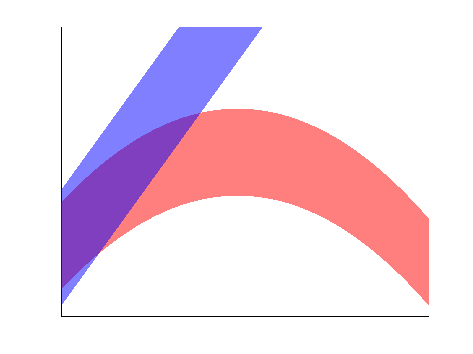
\includegraphics[width=8cm]{mut_wt_vdm_embedding_background}};
%     \node at (0,0)
%       {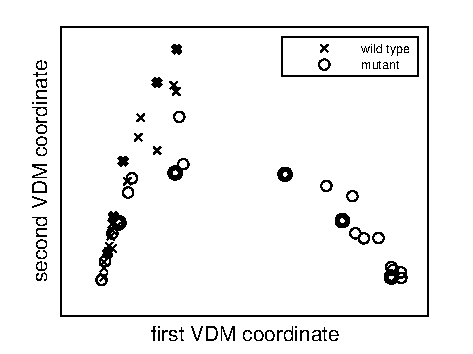
\includegraphics[width=8cm]{mut_wt_vdm_embedding}};
%      \node at (-4cm, 2.4cm) {\textsf{A}};
%\end{tikzpicture}\\
\raisebox{5.2cm}{\textsf{A}}
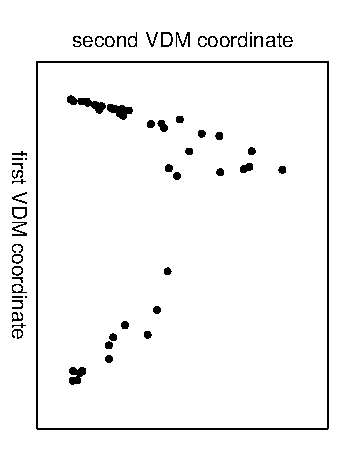
\includegraphics[width=6cm, angle=90]{data3_embed_bw}\\
\raisebox{5.2cm}{\textsf{B}}
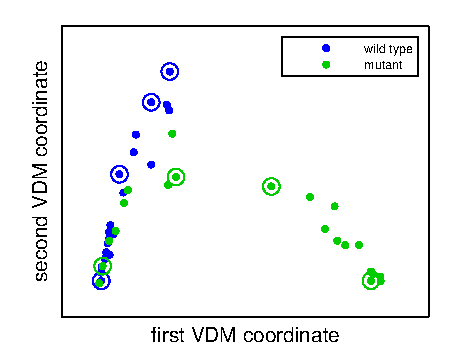
\includegraphics[width=8cm]{data3_embed_color}\\
\begin{tikzpicture}
	\node at (-4.25cm, 0cm) {\textsf{C}};
	\node at (0,0) {
\includegraphics[width=8cm]{wt_trajectory}};
	%\draw[help lines,step=.5] (-4,-1) grid (4,1);
	\draw[->, color=white, thick] (-1.1cm, -0.1cm) -- (-1.3cm, -0.3cm);
	\draw[->, color=white, thick] (-0.7cm, -0.1cm) -- (-0.5cm, -0.2cm);

	\draw[->, color=white, thick] (0.75cm, -0.1cm) -- (0.6cm, -0.3cm);
	\draw[->, color=white, thick] (1.25cm, -0.1cm) -- (1.4cm, -0.3cm);
	
	\draw[->, color=white, thick] (2.8cm, -0.1cm) -- (2.7cm, -0.3cm);
	\draw[->, color=white, thick] (3.3cm, -0.1cm) -- (3.5cm, -0.3cm);

\end{tikzpicture}\\
\begin{tikzpicture}
	\node at (-4.25cm, 0cm) {\textsf{D}};
	\node at (0,0) {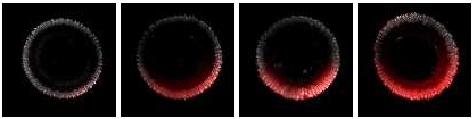
\includegraphics[width=8cm]{mut_trajectory}};

	\draw[->, color=white, thick] (-1cm, -0.2cm) -- (-1cm, -0.5cm);
	
	\draw[->, color=white, thick] (1cm, -0.2cm) -- (1cm, -0.5cm);
	
	\draw[->, color=white, thick] (3cm, -0.2cm) -- (3cm, -0.5cm);

\end{tikzpicture}

\end{document}